\documentclass{article}

\usepackage{fancyhdr}
\usepackage{extramarks}
\usepackage{amsmath}
\usepackage{amsthm}
\usepackage{amsfonts}
\usepackage{tikz}
\usepackage[plain]{algorithm}
\usepackage{algpseudocode}
\usepackage{enumerate}
\usepackage{amsmath}
\usepackage{amssymb}
\usetikzlibrary{automata,positioning}

%
% Basic Document Settings
%

\topmargin=-0.45in
\evensidemargin=0in
\oddsidemargin=0in
\textwidth=6.5in
\textheight=9.0in
\headsep=0.25in

\linespread{1.1}

\pagestyle{fancy}
\lhead{\hmwkAuthorName}
\chead{\hmwkClass\ (\hmwkClassInstructor\ \hmwkClassTime): \hmwkTitle}
\rhead{\firstxmark}
\lfoot{\lastxmark}
\cfoot{\thepage}

\renewcommand\headrulewidth{0.4pt}
\renewcommand\footrulewidth{0.4pt}

\setlength\parindent{0pt}

%
% Create Problem Sections
%

\newcommand{\enterProblemHeader}[1]{
    \nobreak\extramarks{}{Problem \arabic{#1} continued on next page\ldots}\nobreak{}
    \nobreak\extramarks{Problem \arabic{#1} (continued)}{Problem \arabic{#1} continued on next page\ldots}\nobreak{}
}

\newcommand{\exitProblemHeader}[1]{
    \nobreak\extramarks{Problem \arabic{#1} (continued)}{Problem \arabic{#1} continued on next page\ldots}\nobreak{}
    \stepcounter{#1}
    \nobreak\extramarks{Problem \arabic{#1}}{}\nobreak{}
}

\setcounter{secnumdepth}{0}
\newcounter{partCounter}
\newcounter{homeworkProblemCounter}
\setcounter{homeworkProblemCounter}{1}
\nobreak\extramarks{Problem \arabic{homeworkProblemCounter}}{}\nobreak{}

%
% Homework Problem Environment
%
% This environment takes an optional argument. When given, it will adjust the
% problem counter. This is useful for when the problems given for your
% assignment aren't sequential. See the last 3 problems of this template for an
% example.
%
\newenvironment{homeworkProblem}[1][-1]{
    \ifnum#1>0
        \setcounter{homeworkProblemCounter}{#1}
    \fi
    \section{Problem \arabic{homeworkProblemCounter}}
    \setcounter{partCounter}{1}
    \enterProblemHeader{homeworkProblemCounter}
}{
    \exitProblemHeader{homeworkProblemCounter}
}

%
% Homework Details
%   - Title
%   - Due date
%   - Class
%   - Section/Time
%   - Instructor
%   - Author
%

\newcommand{\hmwkTitle}{Tutorial Week 9}
\newcommand{\hmwkDueDate}{March 18, 2021}
\newcommand{\hmwkClass}{CZ4041}
\newcommand{\hmwkClassTime}{CS4}
\newcommand{\hmwkClassInstructor}{Assoc Prof Pan, Sinno Jialin}
\newcommand{\hmwkAuthorName}{\textbf{Pang Yu Shao}}
\newcommand{\hmwkAuthorID}{\textbf{U1721680D}}

%
% Title Page
%

\title{
    \vspace{2in}
    \textmd{\textbf{\hmwkClass:\ \hmwkTitle}}\\
    \normalsize\vspace{0.1in}\small{Due\ on\ \hmwkDueDate\ at 8:30am}\\
    \vspace{0.1in}\large{\textit{\hmwkClassInstructor\ - \hmwkClassTime}}
    \vspace{3in}\\
    \hmwkAuthorName\\
    \hmwkAuthorID
}

\date{18/03/2021}

\renewcommand{\part}[1]{\textbf{\large Part \Alph{partCounter}}\stepcounter{partCounter}\\}

%
% Various Helper Commands
%

% Useful for algorithms
\newcommand{\alg}[1]{\textsc{\bfseries \footnotesize #1}}

% For derivatives
\newcommand{\deriv}[1]{\frac{\mathrm{d}}{\mathrm{d}x} (#1)}

% For partial derivatives
\newcommand{\pderiv}[2]{\frac{\partial}{\partial #1} (#2)}

% Integral dx
\newcommand{\dx}{\mathrm{d}x}

% Alias for the Solution section header
\newcommand{\solution}{\textbf{\large Solution}}

% Probability commands: Expectation, Variance, Covariance, Bias
\newcommand{\E}{\mathrm{E}}
\newcommand{\Var}{\mathrm{Var}}
\newcommand{\Cov}{\mathrm{Cov}}
\newcommand{\Bias}{\mathrm{Bias}}

\begin{document}

\maketitle

\pagebreak

\begin{homeworkProblem}
    Why the condition that the base classifiers should do better than a classifer that performs random
    guessing is necessary for ensemble learning?\\\\



    \textbf{Solution}\\
    Ensemble classifiers perform well when the base classifiers do better than random guessing (i.e., 
    having a error rate of  $ < 50\%$). This is because the ensemble classifier only makes a wrong prediction 
    if the majority of the base classifiers predict incorrectly.\\\\
    When the base classifers have an error rate of more than 50\%, this results in a higher chance of 
    the majority of the classifiers making a wrong prediction -- therefore this causes the ensemble classifier 
    to perform worse than the base classifiers.\\\\

    \begin{displaymath}
        P(N) = \sum^{N}_{i=\frac{N+1}{2}} {N \choose i}\epsilon^i(1-\epsilon)^{N-i}
    \end{displaymath}

    In the example given in the lecture notes, N = 3, and error rate = 0.35
    \begin{displaymath}
        P(3) = {3\choose2}*0.35^2*(1-0.35)^1 + {3\choose3}*0.35^3 
    \end{displaymath}
    \begin{displaymath}
        = 0.28175
    \end{displaymath}
    This performs better than the base classifier, since the error rate of 28\% 
    is less than that of 35\%.

    However, if the base classifier has an error rate of 0.8, we get the following:\\
    \begin{displaymath}
        P(3) = {3\choose2}*0.8^2*(1-0.8)^1 + {3\choose3}*0.8^3 
    \end{displaymath}
    \begin{displaymath}
        = 0.896
    \end{displaymath}

    Therefore, the base classifier should perform better than random guessing in order for 
    ensemble learning to be effective.


\end{homeworkProblem}
\newpage
\begin{homeworkProblem}
    Suppose we have trained 5 base binary classifiers: $f_1$, $f_2$, $f_3$, $f_4$ and $f_5$.
    Their predictions on a validation dataset are shown in Table 1, where the last column
    denotes the ground-truth class labels. Which base classifiers would you choose to construct an 
    ensemble learner.
    \begin{figure}[H]
        \begin{center}
        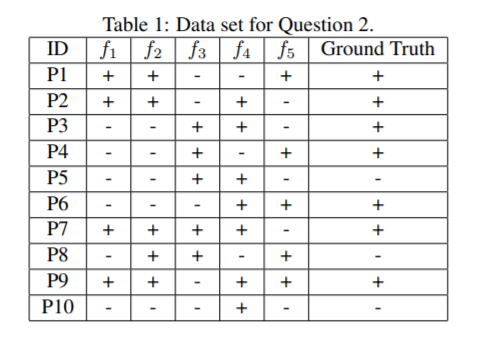
\includegraphics[scale=0.7]{resources/table1.PNG}
        \end{center}
    \end{figure}
    
    \textbf{Solution}\\
    First, get the prediction accuracy of the base classifiers on the dataset:\\
    $f_1: 7/10 = 70\%$\\
    $f_2: 6/10 = 60\%$\\
    $f_3: 4/10 = 40\%$\\
    $f_4: 6/10 = 60\%$\\
    $f_5: 6/10 = 60\%$\\\\

    Since $f_3$ has a prediction accuracy of <50\% it will be excluded from the ensemble learner.\\\\

    It can also be seen that $f_1$ and $f_2$ have the same predictions for 9 out of 10 of the 
    samples. Therefore, it can be suggested that these two classifiers are highly co-related. We 
    exclude $f_2$ from the ensemble since it has a lower prediction accuracy.

    Therefore, the ensemble classifier would be built from $f_1$, $f_4$ and $f_5$.
        

\end{homeworkProblem}



\end{document}